For us, not only the end result was interesting when analysing results from a run, but also the evolvement itself. However, inspecting the evolvement is very interesting, but also complex.

For every generation, there are multiple species, who in turn contain multiple organisms themselves.\cite{Stanley2002}

In our application for inspecting these structures, NEAT\_Visualizer, we can read a JSON dump with logging data from Hippocrates and they will be loaded into the application. The user sees the interfaces as follows:

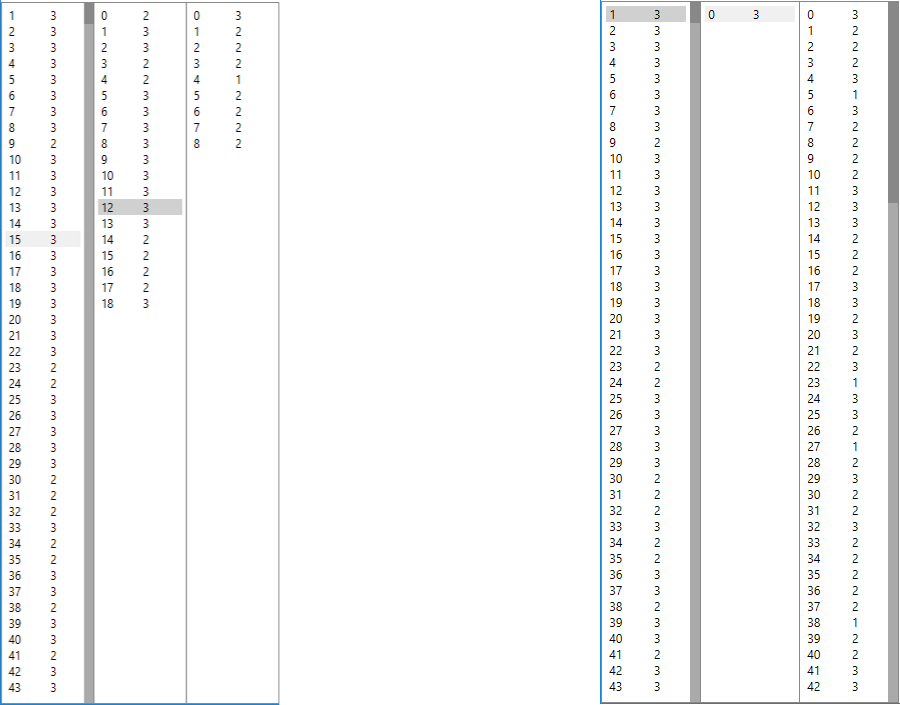
\includegraphics[scale=0.75]{visualizer_gen_complex.png}

Both - the left and the right - views are showing a selected generation, a selected species and no organism selected yet. The control reads from left to right - generation, species, organism.

The numbers are always - left first - Index, then Fitness. As an example, the left picture above has generation 15 with a maximum of 3 fitness selected, and its species number 12 with a maximum fitness of 3.

Here is a full view of the visualizer's graphical user interface (and the network drawing algorithm configured to have all the inputs at the bottom):

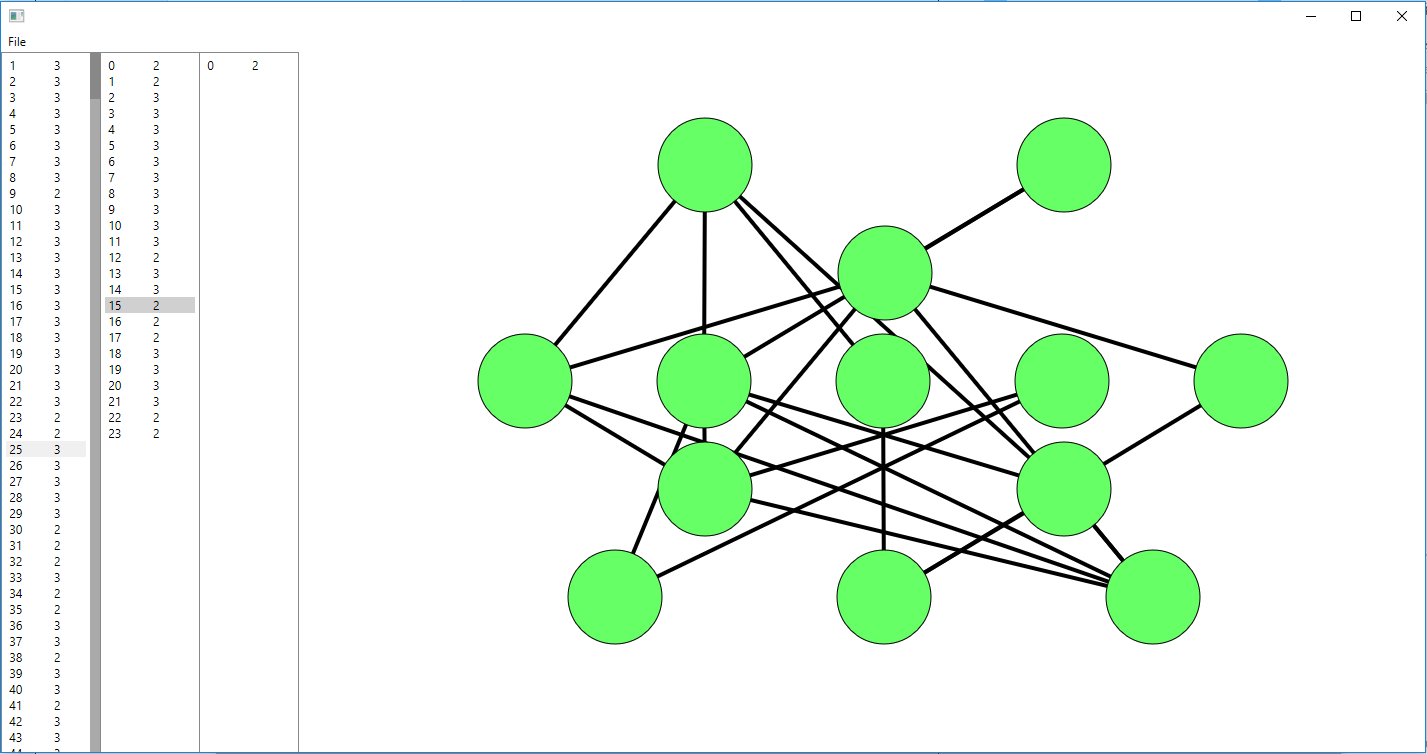
\includegraphics[scale=0.5]{visualizer_full_gui.png}